\documentclass[a4paper]{article}
%\documentclass[a4paper]{book}
\usepackage[utf8]{inputenc}
%\usepackage[italian]{babel}
\usepackage[T1]{fontenc}
\usepackage{amsmath}
\usepackage{physics}
\usepackage{graphicx}
\usepackage{float}
\usepackage{siunitx}
\usepackage{amsfonts}
\usepackage{amssymb}
\usepackage{amsthm}
%\usepackage[export]{adjustbox}
\usepackage{subcaption}
\usepackage{bm}
\usepackage{cancel}
\usepackage{comment}
\usepackage{enumerate}
\usepackage{centernot}

%Comandi da me definiti

\newcommand{\R}{\mathbb{R}}
\newcommand{\C}{\mathbb{C}}

\newcommand{\mat}[1]{\vb{#1}}
\newcommand{\N}{\mathcal{N}}
\newcommand{\e}[1]{\mathrm{e}^{#1}}

\newcommand{\tonde}[1]{\left( {#1} \right)}
\newcommand{\quadre}[1]{\left[ {#1} \right]}
\newcommand{\graffe}[1]{\left\{ {#1} \right\}}
\DeclareMathOperator*{\argmin}{argmin}

\usepackage{xcolor}

\title{Astrostatistics \& Cosmology, exercises 8 to 12}%magari scegli una cosa più carina
\author{Marco Giunta}
\date{\today}

\usepackage{hyperref}
\hypersetup{
    colorlinks=true,
    linkcolor=blue,
    filecolor=magenta,      
    urlcolor=cyan,
    citecolor=blue,%mancava questo! Senza mette il verde di default. O gray
    pdftitle={astrostat exercises 8 to 12 - Marco Giunta},
    bookmarks=true,
    pdfpagemode=FullScreen,
}
\urlstyle{same}

\let\temp\phi%questi comandi scambiano phi e varphi
\let\phi\varphi
\let\varphi\temp

\renewcommand{\L}{\mathcal{L}}%utile perché sono pigro

\renewcommand{\i}{\mathrm{i}} %l'originale è una lettera strana
%non mettere prima questo comando se no non funziona!!
\begin{document}

\maketitle
\tableofcontents

\section{Problem 8}
\subsection{Introduction}
\subsubsection{Matrix notation}
Let's start by setting up proper matrix notation for this problem, as this will pay off later. Notice that our mean data vector $\expval{\vb{y}}$\footnote{Throughout the solution to this problem I set $\vb{y} \equiv \vb{d}$ for reason that will become clear later.} has length $N$, and that as per our model we set it equal to a linear combination of $M$ template vectors $\vb{t}_i$ (each of length $N$, of course), using $M$ coefficients $A_i$ which we want to fit from the data. Mathematically speaking this means:
\begin{equation}
\label{eq:notazione_matriciale}
    \expval{\vb{y}} = \sum_{i=1}^M A_i \vb{t}_i = A_1\vb{t}_1+\dots+A_M\vb{t}_M = \mqty(\vb{t}_1 & \dots & \vb{t}_M)\mqty(A_1\\ \vdots\\ A_M) = \mat{T}\vb{A}
\end{equation}
where $\mat{T}$ is the $N\times M$ matrix where each of the $M$ columns is one of the length-$N$ $\vb{t}_i$ vectors, and $\vb{A}$ is the $\mqty(A_1\ & \dots A_M)^T$ vector of coefficients. The above relation simply exploits the properties of matrix products\footnote{i.e. matrix $\times$ col. vector = l.c. of matrix columns with coefficients equal to the vector components.}, and it gives us a compact way of writing $\expval{\vb{y}}$ while hinting at the need to solve linear systems of equations in order to minimize the $\chi^2$ later on. 
In particular we will show that to solve our problem we need the standard least squares technique from linear algebra, which means solving the unique linear system which ensures L2 norm minimization of some vector.

\subsubsection{Setting up the optimization problem}
Let's assume our prior is uniform, both for simplicity's sake and to actually obtain the $\chi^2$ minimization problem. This means that maximizing the posterior is equivalent to maximizing the likelihood, which we know to be a MVN; this implies our target function is
\begin{equation*}
    P(\vb{A}, \mat{C}|\vb{y}) = \text{const.} \times \exp(-\frac{1}{2}(\vb{y}-\mat{T}\vb{A})^T \mat{C}^{-1} (\vb{y}-\mat{T}\vb{A}) )
\end{equation*}
It then becomes clear that the posterior is maximized when the quantity
\begin{equation*}
    \chi^2 = (\vb{y}-\mat{T}\vb{A})^T \mat{C}^{-1} (\vb{y}-\mat{T}\vb{A})
\end{equation*}
is minimized.\\
The above equation actually forces us to perform another simplification of our problem; indeed notice that in the most general model possible both $\vb{A}$ \emph{and} $\mat{C}$ are parameters,\footnote{Remember that $\vb{y}$ is the fixed dataset, and that the $\mat{T}$ matrix is too since it contains the predetermined templates we want to use to fit $\vb{y}$.} which means that the derivative of $\chi^2$ we'd need to compute would be a complicated tensor with many components. Let us then assume that $\mat{C}$ is known in advance, therefore fixed; in this case we can condition it out of our problem, which is basically equivalent to setting $\chi^2 = \chi^2(\vb{A})$ only.
We conclude that the solution to our problem i.e. the MAP estimator is
\begin{equation*}
    \vb{A}^* = \argmin_{\vb{A}} \chi^2 (\vb{A})
\end{equation*}
What we gain by fixing the covariance matrix is now manifest: it now suffices to compute a simple gradient (of $\chi^2$ w.r.t. the $\vb{A}$ vector) and set it equal to zero to solve our problem.
\begin{equation*}
    \grad\chi^2(\vb{A}^*) = \vb{0}
\end{equation*}


\subsection{Computing $\grad\chi^2$}
We reframed our problem of maximizing the posterior as the problem of computing and setting equal to zero the gradient of $\chi^2$ - which by definition is a \emph{quadratic form of $\vb{A}$}.
There are at least two ways to compute this gradient:
\begin{itemize}
    \item we can either use the vector generalizations of the usual differentiation rules (chain rule, product rule), or
    \item we can compute $\grad\chi^2$ component-wise.
\end{itemize}
The first approach is much quicker, but these rules aren't as widely known as their scalar counterpart; for now, then, let's follow the second one, since standard calculus will suffice (and as a serendipitous side effect we'll discover the vector rules to differentiate a q.f.).\\
We must therefore compute
\begin{equation*}
    (\grad\chi^2)_i = \pdv{A_i}\quadre{(\vb{y}-\mat{T}\vb{A})^T \mat{C}^{-1} (\vb{y}-\mat{T}\vb{A})} = \pdv{A_i} \quadre{\sum_{j,k=1}^N  (\vb{y}-\mat{T}\vb{A})_j C_{jk}^{-1}(\vb{y}-\mat{T}\vb{A})_k}
\end{equation*}
Notice that the last term is the derivative of a sum of many products - each of which is a simple scalar function. Hence by exploiting linearity and the product (Leibniz) rule we obtain:
\begin{equation}
\label{eq:non_lo_so}
    (\grad\chi^2)_i = \sum_{j,k=1}^N \quadre{\pdv{(\vb{y}-\mat{T}\vb{A})_j}{A_i} C_{jk}^{-1} (\vb{y}-\mat{T}\vb{A})_k + (\vb{y}-\mat{T}\vb{A})_j C_{jk}^{-1} \pdv{(\vb{y}-\mat{T}\vb{A})_k}{A_i}}
\end{equation}
Notice that the above quantity is actually the sum of two new quadratic forms, i.e.
\begin{equation}
\label{eq:non_lo_so_2}
    (\grad\chi^2)_i = \pdv{(\vb{y}-\mat{T}\vb{A})^T}{A_i} \mat{C}^{-1}(\vb{y}-\mat{T}\vb{A}) + (\vb{y}-\mat{T}\vb{A})^T \mat{C}^{-1} \pdv{(\vb{y}-\mat{T}\vb{A})}{A_i}
\end{equation}
Either by exploiting the $j\leftrightarrow k$ symmetry in \eqref{eq:non_lo_so} (or equivalently the $\mat{C}^{-1}$ symmetry in \eqref{eq:non_lo_so_2}) we can rewrite the above as

\begin{equation*}
    \pdv{\chi^2}{A_i} = 2 (\vb{y}-\mat{T}\vb{A})^T \mat{C}^{-1} \pdv{(\vb{y}-\mat{T}\vb{A})}{A_i}
\end{equation*}
This derivative is a scalar function; in particular it's a q.f., obtained by a matrix product of the kind (row length $N$ vector) $\times$ ($N\times N$ square matrix) $\times$ (column length $N$ vector). By collecting the $M$ $i=1, \dots, M$ components of the gradient the last term in the above product becomes an $N\times M$ matrix, which means that
\begin{equation}
\label{eq:derivata_vettoriale}
    \grad\chi^2 = 2(\vb{y}-\mat{T}\vb{A})^T \mat{C}^{-1} \grad(\vb{y}-\mat{T}\vb{A})
\end{equation}
must equal a length $M$ row vector - which is correct, given what we know about the $\grad$ operator. Incidentally notice that \eqref{eq:derivata_vettoriale} bears a striking resemblance to 
\begin{equation}
\label{eq:derivata_scalare}
    \dv{f(y)^2}{y} = 2 f(y) \dv{f(y)}{y}
\end{equation}
This of course is no coincidence; indeed we just proved that equation \eqref{eq:derivata_vettoriale} generalizes the well known rule \eqref{eq:derivata_scalare} when $f = \text{a q.f.}$.\\
In order to make 
\begin{equation*}
    \pdv{\chi^2}{A_i} = 2 \sum_{j,k=1}^N (\vb{y}-\mat{T}\vb{A})_j C_{jk}^{-1} \quadre{\pdv{A_i}(\vb{y}-\mat{T}\vb{A})}_k
\end{equation*}
fully explicit, then, the only missing thing is to compute the $k$-th component of
\begin{equation*}
    \pdv{A_i}(\vb{y}-\mat{T}\vb{A}) = \pdv{A_i} \mat{T}\vb{A} = \pdv{A_i}\sum_{\alpha = 1}^M \vb{t}_\alpha A_\alpha = \sum_{\alpha=1}^M \vb{t}_\alpha \pdv{A_\alpha}{A_i} = \sum_{\alpha=1}^M \vb{t}_\alpha \delta_{\alpha i} = \vb{t}_i
\end{equation*}
where we used equation \eqref{eq:notazione_matriciale} plus the usual rules about derivatives.\\
Once again the above result can trivially be rewritten as 
\begin{equation*}
    \grad (\vb{y}-\mat{T}\vb{A}) = \mat{T}
\end{equation*}
since the gradient is a row vector, and since by stacking horizontally the $M$ $\vb{t}_i$ column vectors we recover the definition of the $\mat{T}$ matrix; notice that this result clearly generalizes its 1D counterpart
\begin{equation*}
    \dv{y}(ky+c) = k
\end{equation*}
To recap:
\begin{equation}
\label{eq:gradiente_finale}
    \grad \chi^2 = 2(\vb{y}-\mat{T}\vb{A})^T\mat{C}^{-1}\mat{T}
\end{equation}
Our final result is the following: \emph{setting $\grad\chi^2 = \vb{0}$ is equivalent to solving a system of $M$ homogeneous linear equations}:
\begin{equation}
\label{eq:sistema_vettoriale}
    \grad\chi^2 = \vb{0} \iff (\vb{y}-\mat{T}\vb{A})^T \mat{C}^{-1}\mat{T} = \vb{0}
\end{equation}
which can be explicitly split into its $M$ equations by writing
\begin{equation*}
    (\vb{y}-\mat{T}\vb{A}) \mat{C}^{-1} \vb{t}_i = \sum_{j,k=1}^N (\vb{y}-\mat{T}\vb{A})_j C_{jk}^{-1} (\vb{t}_i)_k = 0 \quad \forall i = 1, \dots, M
\end{equation*}
\subsection{Solving the LSQ linear system}
\subsubsection{How can we find solutions?}
Equation \eqref{eq:sistema_vettoriale} is easily recast into a non homogeneous form as follows:
\begin{equation*}
    (\vb{y}-\mat{T}\vb{A})\mat{C}^{-1}\mat{T} = \vb{0} \implies \vb{y}^T\mat{C}^{-1}\mat{T} - (\mat{T}\vb{A})^T\mat{C}^{-1} \mat{T} = \vb{0}
\end{equation*}
\begin{equation}
\label{eq:sistema_brutto}
    \implies \vb{A}^T \mat{T}^T \mat{C}^{-1}\mat{T} = \vb{y}^T \mat{C}^{-1}\mat{T}
\end{equation}
Now notice we assumed that $\vb{y}$, $\mat{C}$, $\mat{T}$ are all fixed quantities; this means that our linear system is in the form $\vb{A}^T \times \text{const. known matrix} = \text{const. known vector}$. This isn't very practical, since techniques like Gauss' method for linear system assumes the problem to be of the form $\mat{B}\vb{A} = \vb{b}$ for some known $\mat{B}$, $\vb{b}$; this means there are two routes to proceed.
\begin{enumerate}
    \item either we could try to guess some solution, or
    \item we can rewrite our system in an equivalent but friendlier form.
\end{enumerate}
Before moving on to approach \#2 let us explore option \#1 a bit.
\subsubsection{Trivial but useless solutions}
Let us recall that the system we're trying to solve is equivalent to equation \eqref{eq:sistema_vettoriale}. We naturally wonder whether an $\Tilde{\vb{A}}$ such that $\mat{T}\Tilde{\vb{A}} = \vb{y}$ could exist, as a vector with this property would trivially solve our system. Notice that this trivial solution either exists or not depending on $N$ and $M$, since $\mat{T}$ is an $N\times M$ matrix. In particular remember that the Rouché-Capelli theorem states that the number of solutions to the $\mat{T}\Tilde{\vb{A}} = \vb{y}$ system is $\infty^{M-r}$, where $r = \rank\mat{T} \leq N$ is the number of linearly independent equations.
\begin{itemize}
    \item If $M > N (\geq r)$ we have infinite solutions; this makes sense, since it means that we have too many parameters to fit/too few data points to help us fix them. In this case using $\mat{T}\Tilde{\vb{A}}=\vb{t}$ instead of \eqref{eq:sistema_vettoriale} is possible, but nasty since a) we'd like a \emph{general} MAP estimator and b) in practice we would never try to fit e.g. 2000 parameters with only 10 data points.
    \item If $M < (r \leq) N$ we have 0 solutions; once again this makes sense, because it means we have too many independent equations and the parameters can't be set equal to ``agreeing'' values. In this case it's not possible at all to replace \eqref{eq:sistema_vettoriale} with its simpler counterpart.
    \item If $M = N = r$ then $\mat{T}$ is a square, invertible matrix and $\mat{T}\Tilde{\vb{A}}=\vb{y}$ yields the unique, well defined solution $\Tilde{\vb{A}} = \mat{T}^{-1}\vb{y}$. Notice though that this lucky case will never occur in practice, since as explained above one usually chooses models where $N$ is large compared to $M$ (also notice that simply $N=M$ isn't enough, we also need $N=r$; this makes achieving this condition even harder).
\end{itemize}
The above discussion shows that the trivial solution to \eqref{eq:sistema_vettoriale} cannot unfortunately be practically/possibly used in all realistic scenarios; we therefore look for another (arguably better) solution, i.e. one which both always exists (irrespective of $N$, $M$) and that is also unique. These two properties obviously yield a better MAP estimator, which we now show can be obtained by rewriting our original system.

\subsubsection{General \& unique solution}
Notice that by exploiting $\mat{C}^{-1}$'s symmetry we can rewrite \eqref{eq:sistema_vettoriale} with the vector of unknowns on the right. In particular notice that component $i$ of $\grad\chi^2$ equals $2(\vb{y}-\mat{T}\vb{A})^T\mat{C}^{-1}\vb{t}_i$, which is a \emph{scalar} - and hence equals its transpose. By exploiting the property $(\mat{A}\mat{B}\mat{C})^T = \mat{C}^T\mat{B}^T\mat{A}^T$\footnote{See for example \hyperlink{https://math.stackexchange.com/a/795248}{here}.} and $\mat{C}$'s symmetry we obtain:
\begin{equation*}
    (\vb{y}-\mat{T}\vb{A})^T \mat{C}^{-1}\vb{t}_i = \quadre{(\vb{y}-\mat{T}\vb{A})^T \mat{C}^{-1}\vb{t}_i}^T = \vb{t}_i^T (\mat{C}^{-1})^T(\vb{y}-\mat{T}\vb{A})
\end{equation*}
\begin{equation*}
    \implies (\vb{y}-\mat{T}\vb{A})^T \mat{C}^{-1}\vb{t}_i = \vb{t}_i^T \mat{C}^{-1} (\vb{y}-\mat{T}\vb{A})
\end{equation*}
By stacking these scalars in a row we reassemble the gradient, and obtain:
\begin{equation*}
    \grad\chi^2 = (\vb{y}-\mat{T}\vb{A})^T \mat{C}^{-1}\mat{T} = \mat{T}^T \mat{C}^{-1} (\vb{y}-\mat{T}\vb{A})
\end{equation*}
This means equation \eqref{eq:sistema_vettoriale} can be rewritten as
\begin{equation*}
    \mat{T}^T \mat{C}^{-1} (\vb{y}-\mat{T}\vb{A}) = \vb{0}
\end{equation*}
which in turn yields
\begin{equation}
\label{eq:sistema_minimi_quadrati}
    \mat{T}^T \mat{C}^{-1} \mat{T}\vb{A} = \mat{T}^T \mat{C}^{-1}\vb{y}
\end{equation}
as a nice replacement to \eqref{eq:sistema_brutto}. The great thing about \eqref{eq:sistema_minimi_quadrati} is that is satisfies two properties: a) it can be solved with standard techniques since it's in the form $ \text{const. known matrix} \times \vb{A}= \text{const. known vector}$, and b) it's almost identical to the system
\begin{equation}
\label{eq:lsq}
    \mat{D}^T\mat{D}\vb{z} = \mat{D}^T\vb{c}
\end{equation}
The above system is the solution to the least squares problem, i.e. its solution $\Tilde{\vb{z}}$ minimizes the quantity $\norm{\mat{D}\vb{z}-\vb{c}}^2$; since the least square problem always admits a unique solution (which can be found using standard linear algebra techniques to solve linear systems) our MAP estimator will inherit this property. We now proceed to show that \eqref{eq:sistema_minimi_quadrati} always admits a unique, well defined solution - which can then be found by actually solving \eqref{eq:sistema_minimi_quadrati}, e.g. by using Gauss' method.\\
Since $\mat{C}^{-1}$ is an $N\times N$ matrix and $\mat{T}$ is an $N\times M$ one we easily find that $\mat{T}^T \mat{C}^{-1} \mat{T}$ is a square $M\times M$ matrix. As we know a square system always admits a unique solution as long as its matrix is nonsingular; notice that we can assume $\mat{T}^T \mat{C}^{-1} \mat{T}$ is indeed invertible because it's basically impossible that a matrix with ``random'' entries will have $\det = 0$. This must be the case, because if we assume that $\mat{C}$ is fixed by Nature during our experiment we still are in control of the template matrix $\mat{T}$, and one would need to carefully design it in order to ensure $\det( \mat{T}^T \mat{C}^{-1} \mat{T}) = 0$ (and it may be impossible to do so); even if by pure chance one stumbles upon a template matrix capable of setting the determinant equal to zero it would suffice to modify the coefficients inside $\mat{T}$ by a small $\varepsilon$, because this would result in a nonsingular matrix which for all practical purposes is identical to the original one.\\
To recap the above discussion: in general the $\mat{T}^T \mat{C}^{-1} \mat{T}$ will be nonsingular, and even if it is by adding a small $\varepsilon$ somewhere inside $\mat{T}$ we can easily fix that.\\
Therefore we conclude our problem by stating that the unique \& well defined MAP/ML estimator which always exists (irrespectively of $N$, $M$) is the unique solution to the linear system \eqref{eq:sistema_minimi_quadrati}, i.e.
\begin{equation}
\label{eq:soluzione_minimi_quadrati}
    \text{MLE} = (\mat{T}^T \mat{C}^{-1} \mat{T})^{-1}\mat{T}^T\mat{C}^{-1}\vb{x}
\end{equation}
even though in practice it's best to directly solve \eqref{eq:sistema_minimi_quadrati} instead of needlessly (and costly) inverting $\mat{T}^T \mat{C}^{-1} \mat{T}$ as in \eqref{eq:soluzione_minimi_quadrati}.

\section{Problem 9}
\subsection{Introduction}
Once again we have a problem where the likelihood is a MVN. This time we assume that the average is
\begin{equation*}
    \expval{d_i} = \omega x_i + b
\end{equation*}
and the covariance matrix is diagonal but not a multiple of the identity:
\begin{equation*}
    \mat{C} = \mqty(\dmat{\sigma_1^2, \sigma_2^2, \ddots, \sigma_N^2})
\end{equation*}
Notice that if we define $\vb{1} = \mqty(1 & 1 & \dots & 1)^T$ (constant vector of ones) we can rewrite the overall mean as
\begin{equation*}
    \expval{\vb{d}} = \omega \vb{x} + b\vb{1}
\end{equation*}
This equation is interesting because it implies that \emph{we're performing template fitting as in ex. 8}, since we're clearly trying to fit the data as a linear combination of two fixed vectors ($\vb{x}$ and $\vb{1}$) using $M=2$ model parameters ($\omega$ and $b$). If we assume that all errors are known then can recycle equation \eqref{eq:soluzione_minimi_quadrati} and easily obtain our unique and well defined MAP/ML estimator (uniform prior); if instead we assume that the $\mat{C}$ matrix is unknown we first need to marginalize out the $\sigma_i$'s. Let us consider both alternatives and see where they lead us.


\subsection{MAP estimate of $\omega$, $b$ ($\mat{C}$ fixed and known)}
If $\mat{C}$ is known and fixed in advance then we are in the least squares $\chi^2$ minimization situation analyzed in problem 8. In particular in this case we assume:
\begin{equation*}
    \vb{A} = \mqty(\omega \\ b), \ \vb{t}_1 = \vb{x}, \ \vb{t}_2 = \vb{1} \implies \mat{T} = \mqty(\vb{x} & \vb{1}) \implies \mat{T}^T = \mqty(\vb{x}^T \\ \vb{1}^T) = \mqty(x_1 & \dots & x_N \\ 1 & \dots & 1)
\end{equation*}
\begin{equation*}
    \mat{C}^{-1} = \mqty(\dmat{1/\sigma_1^2, \ddots, 1/\sigma_N^2})
\end{equation*}
We have all we need to compute both sides of equation \eqref{eq:sistema_minimi_quadrati} (which is easier to deal with than an explicit matrix inversion as in \eqref{eq:soluzione_minimi_quadrati}).\\
We know that
\begin{equation*}
    \mat{T}\vb{A} = \omega \vb{x}+b\vb{1}
\end{equation*}
This must by multiplied on the left by $\mat{T}^T\mat{C}^{-1}$ to obtain the left hand side of \eqref{eq:sistema_minimi_quadrati}. We obtain:
\begin{equation*}
    \mat{T}^T\mat{C}^{-1}(\mat{T}\vb{A}) = \frac{1}{\sigma_1^2} (\omega x_1+b)\mqty(\vb{x}_1 \\ 1) + \dots + \frac{1}{\sigma_N^2} (\omega x_N+b)\mqty(\vb{x}_N \\ 1) = \sum_{i=1}^N \frac{1}{\sigma_i^2} (\omega x_i+b)\mqty(\vb{x}_i \\ 1)
\end{equation*}
This is true because the fact that $\mat{C}^{-1}$ is diagonal means $\mat{C}^{-1}\mat{T}\vb{A}$ equals the elementwise product of $\mqty(1/\sigma_1^2 & \dots & 1/\sigma_N^2)^T$ and $\omega\vb{x}+b\vb{1}$; therefore the final result equals the linear combination of columns of $\mat{T}^T$ with coefficient equal to the components of this vector. The left hand side is therefore:
\begin{equation*}
    \mat{T}^T\mat{C}^{-1}\mat{T}\vb{A} = \mqty(\sum_{i=1}^N \frac{x_i}{\sigma_i^2}(\omega x_i+b) \\ \sum_{i=1}^N \frac{1}{\sigma_i^2}(\omega x_i+b))
\end{equation*}
\emph{Note:} the above equation already hints at the fact that \emph{we're about to recover the weighted linear regression formulae}. To further stress this fact I prefer to drop the unusual notation $\omega$, $\vb{d}$ in favor of $a$, $\vb{y}$ respectively (i.e. I set $\omega = a$, $\vb{d} = \vb{y}$). Even though it may be potentially confusing/unprofessional to do so halfway there I find it somewhat helpful, so I hope I'll be forgiven.\\
We now find the right hand side of the system to be solved:
\begin{equation*}
    \mat{T}^T\mat{C}^{-1}\vb{y} = \mqty(x_1 & \dots & x_N \\ 1 & \dots & 1)\mqty(y_1/\sigma_1^2 \\ \vdots \\ y_N/\sigma_N^2) = \sum_{i=1}^N \frac{y_i}{\sigma_i^2}\mqty(x_i \\ 1) = \mqty(\sum_i \frac{y_i x_i}{\sigma_i^2} \\ \sum_i \frac{y_i}{\sigma_i^2})
\end{equation*}
By comparing the two sides of the equation we find that our system is indeed made up of $M=2$ unknowns and equations:
\begin{equation*}
    \begin{cases}
        \sum_i \quadre{ a \frac{x_i^2}{\sigma_i^2} + b\frac{x_i}{\sigma_i^2}}= \sum_i \frac{y_i x_i}{\sigma_i^2}\\
        \sum_i \quadre{a \frac{x_i}{\sigma_i^2} + b \frac{1}{\sigma_i^2}} = \sum_i \frac{y_i}{\sigma_i^2}
    \end{cases}
\end{equation*}
Notice that our unknowns $a$, $b$ do not depend on $i$ - hence we can collect the sums.
\begin{equation*}
    \begin{cases}
        \quadre{\sum_i (x_i/\sigma_i)^2}a + \quadre{\sum_i x_i/\sigma_i^2}b = \quadre{\sum_i x_iy_i/\sigma_i^2}\\
        \quadre{\sum_i x_i/\sigma_i^2} a + \quadre{\sum_i 1/\sigma_i^2}b = \quadre{\sum_i y_i/\sigma_i^2}
    \end{cases}
\end{equation*}
This can be rewritten in matrix form as 
\begin{equation}
\label{eq:sistema_pesato}
    \mqty(\sum_i (x_i/\sigma_i)^2 & \sum_i x_i/\sigma_i^2 \\ \sum_i x_i/\sigma_i^2 & \sum_i 1/\sigma_i^2)\mqty(a \\ b) = \mqty(\sum_i x_iy_i/\sigma_i^2 \\ \sum_i y_i/\sigma_i^2)
\end{equation}
This is a $2\times 2$ matrix, which is easily inverted - or equivalently we can solve the system using Cramer's rule.\footnote{It's easy to check that the determinant is nonzero.} In particular we know that given the $2\times 2$ linear system
\begin{equation*}
    \mqty(a & b \\ c & d)\mqty(x \\ y) = \mqty(e \\f), \quad ad-bc \neq 0
\end{equation*}
its solution is:
\begin{equation*}
    \begin{cases}
        x = \frac{ed-bf}{ad-bc} \\
        y = \frac{af-ec}{ad-bc}
    \end{cases}
\end{equation*}
In our case we finally find:
\begin{equation*}
    a = \frac{\tonde{\sum_{i=1}^N \frac{x_i y_i}{\sigma_i^2}} \tonde{\sum_{i=1}^N \frac{1}{\sigma_i^2}} - \tonde{\sum_{i=1}^N \frac{x_i}{\sigma_i^2}}\tonde{\sum_{i=1}^N \frac{y_i}{\sigma_i^2}}}{\quadre{\sum_{i=1}^N \tonde{\frac{x_i}{\sigma_i}}^2}\tonde{\sum_{i=1}^N \frac{1}{\sigma_i^2}} - \tonde{\sum_{i=1}^N \frac{x_i}{\sigma_i^2}}^2}
\end{equation*}
\begin{equation*}
    b = \frac{\quadre{\sum_{i=1}^N \tonde{\frac{x_i}{\sigma_i}}}^2 \tonde{\sum_{i=1}^N \frac{y_i}{\sigma_i^2}} - \tonde{\sum_{i=1}^N \frac{x_i y_i}{\sigma_i^2}}\tonde{\sum_{i=1}^N \frac{x_i}{\sigma_i^2}}}{\quadre{\sum_{i=1}^N \tonde{\frac{x_i}{\sigma_i}}^2}\tonde{\sum_{i=1}^N \frac{1}{\sigma_i^2}} - \tonde{\sum_{i=1}^N \frac{x_i}{\sigma_i^2}}^2}
\end{equation*}
These are indeed the weighted linear regression formulae, the ones we can obtain if we try to fit $N$ points $(x_i, y_i)$ to the $y = ax + b$ line if we give to each point a $1/\sigma_i^2$ weight (i.e. more accurate points weigh more).\\ 
Of course if we set $\sigma_i = \sigma \ \ \forall i$ we recover the non weighted case formulae:
\begin{equation}
\label{eq:a_non_pesato}
    a = \frac{N \sum_i x_i y_i - \tonde{\sum_i x_i}\tonde{\sum_i y_i}}{N\sum_i x_i^2 - \tonde{\sum_i x_i}^2}
\end{equation}
\begin{equation}
\label{eq:b_non_pesato}
    b = \frac{\tonde{\sum_i x_i^2}\tonde{\sum_i y_i} - \tonde{\sum_i x_i y_i}\tonde{\sum_i x_i}}{N\sum_i x_i^2 - \tonde{\sum_i x_i}^2}
\end{equation}

\subsection{MAP estimate of $\omega$, $b$ ($\mat{C}$ unknown and not fixed)}
%fai vedere che si arriva sempre al minimizzare il chi quadro --> the "reliable" unique and well defined solution can be found by solving the system... notice that it's well defined since r=2 per la linear ind., la sol banale non va perché M=2 e N>2....
% se non marginalizzo perché conosco le sigma vuol dire che la mia soluzione le potrà contenere --> regressione pesata. se non le conosco e di conseguenza marginalizzo la mia soluzione non potrà mai essere la regressione non pesata - e in effetti ottengo il sistema lineare sovra determinato semplice che ho ottenuto prima. Nota: prima era inutile perché volevo una soluzione non ai minimi quadrati e conoscevo C, ora almeno nel caso di C sconosciuta mi devo accontentare di una soluzione ai minimi quadrati (quindi sarebbe tornare indietro e ridare un po' di dignità a quel sistema). inoltre nota che è bello che quando marginalizzo la regressione ritorni non pesata; in effetti se non so nulla sugli errori sembra democratico dare a tutte le componenti di x lo stesso peso (anche se dovrei riflettere sul se questo segua direttamente dal prior uniforme sulle sigma)
Let us now consider the case where the $\sigma_i$ are \emph{not} known beforehand; in this case we clearly cannot make use of ex. 8's results, and we have to start over the same standard procedure.\\
To solve the problem we once again start with a uniform prior assumption, which implies that likelihood and posterior are the same up to a constant. The resulting posterior will be a function of $a$, $b$ and $\mat{C}$; in order to find MAP estimates of $a$, $b$ we first need to marginalize out the $\sigma_i$'s. Notice that this will of course make the $\sigma_i$'s disappear from our final result, since this time they're just nuisance parameters; this in turn means that \emph{we can no longer recover the \emph{weighted} linear regression formulae}. This makes sense: this time we cannot assign a weight to each point beforehand, so we expect the final equations to be those of simple linear regression.\\
Given that the covariance matrix is diagonal one easily finds:\footnote{Notice that in this case $\sqrt{\det\mat{C}} = \sqrt{\prod_i \sigma_i^2} = \prod_i \sigma_i$ since $\mat{C}$ is diagonal.}
\begin{equation*}
    P(\vb{A}|\vb{y}) = \int_{\R_+^N} \dd[N]{\vb*{\sigma}} P(\vb{A}, \vb*{\sigma}|\vb{y}) \propto \int_{\R_+^N} \dd[N]{\vb*{\sigma}} \frac{1}{\prod_{i=1}^N \sigma_i}\exp(-\sum_{i=1}^N \tonde{\frac{(\vb{y}-\mat{T}\vb{A})_i}{\sigma_i \sqrt{2}}}^2)
\end{equation*}
where we defined $\vb*{\sigma}$ as the vector containing the $\sigma_i$'s (each of which is of course a positive number).
Let us define $\vb{h} = \vb{y} - \mat{T}\vb{A}$ to simplify the notation a bit. With a bit of work our integral becomes equal to:
\begin{equation*}
    I \equiv \prod_{i=1}^N \int_0^{+\infty} \dd{\sigma_i} \frac{1}{\sigma_i} \exp(-\frac{h_i^2}{2\sigma_i^2})
\end{equation*}
where we simply paired each $\sigma_i$ with one exponential before multiplying everything.
We now change variables using $\alpha_i \equiv 1/\sigma_i \implies \dd{\alpha_i} = -\dd{\sigma_i}/\sigma_i^2$. We find:\footnote{The minus sign brought by the differential cancels the swap of integration bound.}
\begin{equation*}
    I = \prod_{i=1}^N \int_0^{+\infty} \dd{\alpha_i} \alpha_i \exp(-\frac{h_i^2}{2}\alpha_i^2 )
\end{equation*}
Thanks to \hyperlink{https://en.wikipedia.org/wiki/Gaussian_integral}{this page} we know that
\begin{equation*}
    \int_0^{+\infty} x \mathrm{e}^{-bx^2}\dd{x} = \frac{1}{2b}
\end{equation*}
By using this result we can compute
\begin{equation*}
    I = \frac{1}{2} \prod_{i=1}^N \frac{2}{h_i^2} \propto \prod_{i=1}^N h_i^{-2}
\end{equation*}
To remove that nasty product we can consider the log posterior. We find:
\begin{equation*}
    \log P(\vb{A}|\vb{y}) = \sum_{i=1}^N \log(h_i^{-2}) + \text{const.} = -\sum_{i=1}^N \log(h_i^2) + \text{const.}
\end{equation*}
\begin{equation*}
    \implies \mathrm{argmax} \ P(\vb{A}|\vb{y}) = \argmin \sum_{i=1}^N \log h_i^2
\end{equation*}
Now we notice that since the logarithm is a monotonically increasing function we can write:
\begin{equation*}
    \argmin \sum_{i=1}^N \log h_i^2 = \argmin \sum_{i=1}^N h_i^2 = \argmin \sum_{i=1}^N (\vb{y}-\mat{T}\vb{A})_i^2
\end{equation*}
This means that our solution is:
\begin{equation*}
    \vb{A}^* = \argmin_{\vb{A}} \norm{\vb{y} - \mat{T}\vb{A}}^2
\end{equation*}
The fact that $\mat{T}\vb{A} = a\vb{x}+b\vb{1}$ tells us some interesting results about the previous equation. In particular:
\begin{itemize}
    \item We recovered simple linear regression: indeed we found that our MAP estimates for $a$, $b$ minimize the squared difference between each of the observed $y_i$ and its expected value $\hat{y}_i = ax_i+b$ (i.e. the squared norm of the $\vb{y} - \hat{\vb{y}} = \vb{y}-\mat{T}\vb{A}$ vector). This is exactly the least squares method application usually carried out to derive simple linear regression formulae.
    \item The fact that we found a least squares solution guarantees that the solution exists and is unique; e.g. if we had found that our MAP estimators had to specifically satisfy $\vb{y}-\mat{T}\vb{A} = \vb{0}$ we would have found no solution to our problem. This follows from the discussion carried out in problem 8 ($\mat{T}\vb{A} = \vb{y}$ has 0 solutions when $M<N$, which is our case since $M=2<N$), but can also be rederived on the spot by observing that $\mat{T}\vb{A}=\vb{y}$ is equivalent to $ax_i+b=y_i \ \forall i$, which is a system with 0 solutions due to experimental error.\footnote{This last statement is true both in the sense that at best $ax_i+b\approx y_i$ only, and also in the sense that in general the $N$ equations will be independent - hence making the system ``too rich'', since many equations for just two unknowns are incompatible.}
\end{itemize}
We already reminded ourselves that the unique vector which minimizes $\vb{h}$'s squared norm is the only solution to the system outlined in equation \eqref{eq:lsq}; from this point on we simply repeat the standard linear regression equations derivation/a simplified version of the weighted derivation carried out above.\\
Indeed if we compute the matrix products we obtain the system
\begin{equation*}
    \mqty(\sum_i x_i^2 & \sum_i x_i \\ \sum_i x_i & N)\mqty(a \\ b) = \mqty(\sum_i x_iy_i \\ \sum y_i)
\end{equation*}
This is the same system as in \eqref{eq:sistema_pesato} but with $\sigma_i$ replaced with the same constant $\forall i$, which means that our final solution is the same as in equations \eqref{eq:a_non_pesato} and \eqref{eq:b_non_pesato}.
This concludes this part of the exercise.\\
\emph{One final remark} notice how swapping the delta prior\footnote{Conditioning w.r.t. $\mat{C}$ is equivalent to marginalizing the posterior using a delta prior for $\mat{C}$, as one can easily show.} for the $\sigma_i$'s with a uniform one impacted the result: removing this extra knowledge made the final solution less precise, in the sense that each measurement is given the same weight - and as we know this is sub optimal if some points ``deserve'' more weight in determining the best estimates.

\subsection{ML estimate of $\mat{C}$}
%l'altra marginalizzazione, l'integrale ha la stessa integranda ma cambia la variabile di integrazione che adesso manca al di fuori dell'esponente. Occhio però allo jacobiano se ti vuoi sbarazzare della traslazione!
Let's now turn our attention to the problem of computing the MAP estimator for $\mat{C}$ (equivalently: for the $\vb*{\sigma} = (\sigma_i)$ vector). In principle we need to perform the same two-step procedure as above: marginalize w.r.t. $(a,b)$, then maximize the resulting function. This unfortunately is impractical; not only do we need to perform a \emph{double} integral this time (which can still be evaluated analytically), but the result is a very complicated function of $\sigma_i$ (which is hard/impossible to differentiate analytically).\footnote{At least according to my own calculations, which may still be wrong.}\\
Since we would have used a uniform prior anyway (hence giving up one of the advantages of Bayesian statistics over the frequentist one) let us compute a ML estimator instead of a MAP one. In practice this means that our estimator for $\vb*{\sigma}$ must be computed by maximizing the likelihood \emph{with $a$, $b$ substituted respectively with their ML(/MAP) estimators $\hat{a}$, $\hat{b}$ computed before}. We therefore maximize:
\begin{equation*}
    \hat{\L}(D|\vb*{\sigma}) \propto \frac{1}{\sqrt{\prod_i \sigma_i}} \exp(-\frac{1}{2}\sum_{i=1}^N \frac{(y_i - \hat{a}x_i - \hat{b})^2}{\sigma_i^2})
\end{equation*}
This lets us appreciate why Bayesian statistics is often better than its frequentist counterpart; indeed notice that in the previous equation we're sticking to a single model ($a = \hat{a}$, $b = \hat{b}$) instead of naturally incorporating the uncertainty over $a$, $b$ via marginalization. Exclusively using the best model available may lead to unaccurate predictions, and has the problem that there is no natural/standard way to estimate uncertainties; Bayesian statistics, instead, makes use of probability theory to reach results that \emph{ad hoc} methods cannot.\\
Having said that we compute the logarithm of $\hat{\L}$ for simplicity, hence obtaining
\begin{equation*}
    \ln\hat{L}(D|\vb*{\sigma}) = \text{const.} - \frac{1}{2}\ln(\prod_i \sigma_i^2) - \frac{1}{2} \sum_{i=1}^N \frac{(y_i - \hat{a}x_i - \hat{b})^2}{\sigma_i^2}
\end{equation*}
which can be rewritten as
\begin{equation}
    \ln\hat{L}(D|\vb*{\sigma}) = \text{const.} - \sum_{i=1}^N \ln \sigma - \frac{1}{2} \sum_{i=1}^N \frac{(y_i - \hat{a}x_i - \hat{b})^2}{\sigma_i^2}
\end{equation}
We can now easily compute the derivative:
\begin{equation*}
    \pdv{\sigma_j} \ln\hat{L} = -\frac{1}{\sigma_j} + \frac{(y_i - \hat{a}x_i - \hat{b})^2}{\sigma_i^3}
\end{equation*}
By setting this equal to zero we immediately find our estimator for each of $\vb*{\sigma}$'s components.
\begin{equation*}
    \hat{\sigma}_i^2 = (y_i - \hat{a}x_i - \hat{b})^2
\end{equation*}
or equivalently:
\begin{equation*}
    \hat{\sigma}_i = \abs{y_i - \hat{y}_i}
\end{equation*}
where $\hat{y}_i$ is our unbiased estimator for $\expval{y}_i$. The result we just obtained is quite intuitive: indeed we found that the empirical error $\abs{y_i - \hat{y}_i}$ can be used as an estimator for the theoretical error.\\
Another way to understand why this result is intuitive is to consider the case $\sigma_i = \sigma \ \forall i$, in which case we can easily prove that $\hat{\sigma}_i^2$ is the usual frequentist estimator for the variance of a gaussian. Indeed we easily obtain:
\begin{equation*}
    \ln\hat{\L} = \text{const.} - N\ln\sigma - \frac{1}{2\sigma^2}\text{RSS}
\end{equation*}
\begin{equation*}
    \eval{\dv{\ln\hat{L}}{\sigma}}_{\hat{\sigma}} = \eval{\tonde{-\frac{N}{\sigma} + \frac{\text{RSS}}{\sigma^3}}}_{\hat{\sigma}} = 0
\end{equation*}
\begin{equation*}
    \hat{\sigma}^2 = \frac{\text{RSS}}{N} = \frac{1}{N} \sum_{i=1}^N (y_i-\hat{y}_i)^2 = \text{MSE}
\end{equation*}
which indeed is the classic gaussian variance frequentist estimator.

%\subsection{Solution recap: weighted linear regression formulae} %inutile


\section{Problem 10}
\subsection{Introduction}
Up to some constants it's easy to see that our likelihood is the exponential of $-\text{RSS}/(2\sigma^2)$, where
\begin{equation*}
    \text{RSS} = \sum_{i=1}^N \tonde{d_i - \beta_0 -\sum_{j=1}^p \beta_j x_{ij}}^2
\end{equation*}
If we use a uniform prior MAP = MLE, which means that our MAP estimator is clearly the one which minimizes the RSS.\\
If instead we want to use a different prior we must maximize a different posterior, which in turn modifies our MAP estimator.
\subsection{Laplace Prior}
A double exponential/Laplace prior is:
\begin{equation*}
    \beta_i \sim \frac{1}{2b}\exp(-\frac{\abs{\beta_i}}{b}) \qquad \forall i = 0,\dots, p
\end{equation*}
If we assume all $\beta_j$ are i.i.d. we can write the overall prior as
\begin{equation*}
    P(\vb*{\beta}) = \prod_{j=0}^p \frac{1}{2b}\exp(-\frac{\abs{\beta_j}}{b}) = \tonde{\frac{1}{2b}}^{p+1}\exp(-\frac{1}{b}\sum_{j=0}^p \abs{\beta_j})
\end{equation*}
This yields the following posterior:
\begin{equation*}
    P(\vb*{\beta}|D,I) \propto \exp(-\frac{1}{2\sigma^2}\sum_{i=1}^N \tonde{d_i - \beta_0 -\sum_{j=1}^p \beta_j x_{ij}}^2)\exp(-\frac{1}{b}\sum_{j=0}^p \abs{\beta_j})
\end{equation*}
We can rewrite this as 
\begin{equation*}
    P(\vb*{\beta}|D,I) \propto \exp(-\frac{1}{2\sigma^2}\quadre{\underbrace{\sum_{i=1}^N \tonde{d_i - \beta_0 -\sum_{j=1}^p \beta_j x_{ij}}^2}_{= \text{RSS}} + \frac{2\sigma^2}{b}\sum_{j=0}^p \abs{\beta_j}})
\end{equation*}
From this we trivially obtain:
\begin{equation*}
    \hat{\vb*{\beta}} = \text{argmin} \tonde{\text{RSS} + \frac{2\sigma^2}{b}\sum_{j=0}^p \abs{\beta_j}}
\end{equation*}
which is the L1 regularization we were supposed to find.

\subsection{Gaussian prior}
This time we assume the following prior:
\begin{equation*}
    \beta_i \sim \mathcal{N}(0,c) \propto \exp(-\frac{\beta_i^2}{2c^2})
\end{equation*}
Once again we assume i.i.d. sampling to write down the full prior as:
\begin{equation*}
    P(\vb*{\beta}|I) \propto \prod_{j=0}^p \exp(-\frac{\beta_j^2}{2c^2}) = \exp(-\frac{1}{2c^2}\sum_{j=0}^p \beta_j^2) = \exp(-\frac{1}{2\sigma^2} \frac{\sigma^2}{c^2}\sum_{j=0}^p \beta_j^2)
\end{equation*}
Proceeding as above one we find:
\begin{equation*}
    \hat{\vb*{\beta}} = \text{argmin} \tonde{\text{RSS} + \frac{\sigma^2}{c}\sum_{j=0}^p \beta_j^2}
\end{equation*}
which is the L2 regularization we were supposed to find.


\section{Problem 11}
\subsection{Introduction}
We start by noting that our model consists of a MVN likelihood depending on $n+1$ parameters: a length $n$ vector ($\vb*{\theta}$) and a single scalar ($A$). In particular we can write down the full likelihood as:
\begin{equation*}
    \L(\vb{x}|\vb*{\theta}, A) = \frac{1}{(2\pi)^{N/2}\sqrt{\det \mat{C}}}\exp(-\frac{1}{2}(\vb{x} - A\overline{\vb{x}})^T \mat{C}^{-1}(\vb{x} - A\overline{\vb{x}}))
\end{equation*}
where $\overline{\vb{x}} = \overline{\vb{x}}(\vb*{\theta})$, i.e. the expected value of $\vb{x}$ is a function of the $\vb*{\theta}$ vector of parameters - and this mean is further rescaled by the $A$ parameter.

\subsection{Marginalization to remove $A$}
In order to marginalize $A$ out we first need to obtain the posterior, i.e. an actual pdf for $A$. Once we obtain the posterior we simply need to compute the marginalized posterior using
\begin{equation*}
    \underbrace{P(\vb*{\theta}|\vb{x})}_{\text{marginalized post.}} = \int_{-\infty}^{+\infty} \underbrace{P(\vb*{\theta},A|\vb{x})}_{\text{overall post.}} \dd{A}
\end{equation*}
where in the above we assumed $A\in\R$, i.e. $A$ is free to range from $-\infty$ to $+\infty$.\\
The above in turn implies we need a prior for \emph{all} model parameters, not just $A$; if we further assume all model parameters are independent and for all of them we use a uniform prior we simply have
\begin{equation*}
    P(\vb*{\theta},A|\vb{x}) = \frac{1}{Z}\L(\vb{x}|\vb*{\theta}, A)
\end{equation*}
where $Z$ is the evidence, i.e. the normalization constant obtained by integrating the likelihood w.r.t. all model parameters.\\
The marginalized posterior must therefore be
\begin{equation*}
    P(\vb*{\theta}|\vb{x}) = K \int_{-\infty}^{+\infty} \dd{A} \exp(-\frac{1}{2}(\vb{x} - A\overline{\vb{x}})^T \mat{C}^{-1}(\vb{x} - A\overline{\vb{x}}))
\end{equation*}
where $K^{-1} \equiv Z (2\pi)^{N/2} \sqrt{\det\mat{C}}$. Notice that $\vb{x}$, $\overline{\vb{x}}(\vb*{\theta})$ and $\mat{C}$ are all $A$-independent quantities, and can therefore be treated as constants. If we expand the argument of the exponential we obtain:
\begin{equation*}
    -\frac{1}{2}\quadre{\vb{x}^T\mat{C}^{-1}\vb{x} - \vb{x}^T\mat{C}^{-1}A\overline{\vb{x}} - A\overline{\vb{x}}^T \mat{C}^{-1}\vb{x} + A^2 \overline{\vb{x}}^T \mat{C}^{-1} \overline{\vb{x}}} = -\frac{1}{2}\quadre{aA^2 + 2bA + c}
\end{equation*}
where we defined $a \equiv \overline{\vb{x}}^T \mat{C}^{-1} \overline{\vb{x}}$, $b \equiv - \vb{x}^T\mat{C}^{-1}\overline{\vb{x}}$, $c\equiv \vb{x}^T \mat{C}^{-1}\vb{x}$ and exploited the symmetry of $\mat{C}^{-1}$ to write
\begin{equation*}
    (\vb{x}^T\mat{C}^{-1}\overline{\vb{x}})^T = \overline{\vb{x}}^T(\mat{C}^{-1})^T\vb{x} = \overline{\vb{x}}^T\mat{C}^{-1}\vb{x} \implies \vb{x}^T\mat{C}^{-1}\overline{\vb{x}} + \overline{\vb{x}}^T\mat{C}^{-1}\vb{x} = 2\vb{x}^T\mat{C}^{-1}\overline{\vb{x}} = -2b
\end{equation*}
Our marginalized posterior becomes:
\begin{equation*}
    P(\vb*{\theta}|\vb{x}) = D \int_{-\infty}^{+\infty} \exp(-\frac{1}{2}(aA^2+bA))
\end{equation*}
where $D\equiv K \exp(-c/2)$. This integral is easily computed; indeed it suffices to refer to the identity
\begin{equation*}
    \int_{\R^n} \exp[-\frac{1}{2}\vb{y}^T\mat{A}\vb{y} +\vb{b}^T \vb{y}] \dd[n]{\vb{y}} = \frac{(2\pi)^{n/2}}{\sqrt{\det\mat{A}}}\exp(\frac{1}{2}\vb{b}^T \mat{A}^{-1}\vb{b})
\end{equation*}
which can be tailored to the problem at hand by setting $n=1$, $\vb{y} = A$, $\vb{b} = b$, $\mat{A} = a$.\\
We find:
\begin{equation*}
    P(\vb*{\theta}|\vb{x}) = D \sqrt{\frac{2\pi}{a}}\exp(\frac{b^2}{2a})
\end{equation*}
where $a = \overline{\vb{x}}^T \mat{C}^{-1} \overline{\vb{x}}$, $b = - \vb{x}^T\mat{C}^{-1}\overline{\vb{x}}$, and $D$ are all fuctions of $\overline{\vb{x}}(\vb*{\theta})$ - hence of $\vb*{\theta}$.

\section{Problem 12}
\subsection{12.1: $\L$ computation}
If we assume statistical independence for our dataset $D = \{d_i\}_{i=1}^N$ we can write
\begin{equation*}
    \L(D|\omega, B_1, B_2, I) = \prod_{i=1}^N \L(d_i|\omega, B_1, B_2, I)
\end{equation*}
i.e. we can obtain the overall likelihood as the product of the $N$ single-datum functions. Notice that each of these is a gaussian, as dictated by the chosen model; in particular since $d_i = f(t_i)+\varepsilon_i$, $\epsilon_i\sim \mathcal{N}(d_i-f(t_i), \sigma^2)$ (with $\sigma^2$ known in advance) we can write:
\begin{equation*}
    \L(d_i|\omega, B_1, B_2, I) = \frac{1}{\sigma \sqrt{2\pi}}\exp(-\frac{1}{2\sigma^2} (d_i-B_1\cos(\omega t_i)-B_2\sin(\omega t_i))^2)
\end{equation*}
Thanks to the properties of exponential we therefore obtain:
\begin{equation*}
    \L(D|\omega, B_1, B_2, I) = \frac{1}{\sigma^N (2\pi)^{N/2}}\exp(-\frac{1}{2\sigma^2} \sum_{i=1}^N (d_i-B_1\cos(\omega t_i)-B_2\sin(\omega t_i))^2)
\end{equation*}
We know expand the $(\dots)^2$ term in the sum using the identity
\begin{equation}
\label{eq:quadrato_trinomio}
    (a+b+c)^2 = a^2 + b^2 + c^2 + 2ab + 2ac + 2bc
\end{equation}
Once this expansion is carried out if we sum over $i$ we obtain six terms that if multiplied by $-1/(2\sigma^2)$ make up the exponent. In particular we're stating that it's possible to write
\begin{equation*}
    \L(D|\omega, B_1, B_2, I) = \frac{1}{\sigma^N (2\pi)^{N/2}}\exp(-\frac{Q}{2\sigma^2})
\end{equation*}
where $Q$ is the sum of six terms obtained as shown in \eqref{eq:quadrato_trinomio}.\\
We obtain:
\begin{equation*}
    Q = \sum_{i=1}^N \tonde{d_i^2 + B_1^2\cos^2(\omega t_i)+ B_2^2\sin^2(\omega t_i)-2d_iB_1\cos(\omega t_i) -2d_iB_2\sin(\omega t_i) + 2B_1B_2\cos(\omega t_i)\sin(\omega t_i)}
\end{equation*}

\begin{align*}
    = \tonde{\sum_{i=1}^N d_i^2} - 2 &\tonde{B_1\sum_{i=1}^N d_i \cos(\omega t_i) + B_2 \sum_{i=1}^N d_i\sin(\omega t_i)} + \tonde{B_1^2 \sum_{i=1}^N \cos^2(\omega t_i)} + \tonde{B_2^2 \sum_{i=1}^N \sin^2(\omega t_i)} +\\
    &+\tonde{2 B_1 B_2 \sum_{i=1}^N \cos(\omega t_i) \sin(\omega t_i)}
\end{align*}
where in the last step we conveniently collected terms.\\
Notice that the first term can be rewritten as
\begin{equation*}
    \sum_{i=1}^N d_i^2 = N \tonde{\frac{1}{N}\sum_{i=1}^N d_i^2} = N \overline{d^2}
\end{equation*}
whereas the others can be rewritten by defining the following functions:
\begin{equation*}
    R(\omega) = \sum_{i=1}^N d_i \cos(\omega t_i)
\end{equation*}
\begin{equation*}
    I(\omega) = \sum_{i=1}^N d_i \sin(\omega t_i)
\end{equation*}
\begin{equation*}
    c(\omega) = \sum_{i=1}^N \cos^2(\omega t_i)
\end{equation*}
\begin{equation*}
    s(\omega) = \sum_{i=1}^N \sin^2(\omega t_i)
\end{equation*}
\begin{equation*}
    a(\omega) = \sum_{i=1}^N \cos(\omega t_i) \sin(\omega t_i)
\end{equation*}
Each of these can be considered a function of the model parameter $\omega$ (since we consider the dataset fixed); for brevity's sake in the what follows we'll sometimes omit the argument.\\
We can now rewrite $Q$ as follows:\footnote{Notice that the problem sheet failed to list the $a$ term; luckily this doesn't invalidate the problem's main results, as we will show later that $a$ is negligible under the high frequency approximation.}
\begin{equation*}
    Q = N\overline{d^2} - 2(B_1 R + B_2 I) + B_1^2 c + B_2^2 s + 2 B_1B_2 a
\end{equation*}
which concludes point 12.1.

\subsection{12.2: Proof that $c(\omega)$, $s(\omega)$, $a(\omega) \approx \text{const.}$}
Let's start by computing an approximation for $c(\omega)$. We first notice that under appropriate assumptions we can write:
\begin{equation*}
    c(\omega) = \sum_{i=1}^N \cos^2(\omega t_i) = N \tonde{\frac{1}{N}\sum_{i=1}^N \cos^2(\omega t_i)}\approx N \expval{\cos^2 (\omega t)}
\end{equation*}
To explain why the above holds let's make the following assumptions:
\begin{itemize}
    \item we assume that the observation time during which the data was collected has a fixed length, i.e. $N=1/\Delta$ (if the $[t_1, t_N]$ interval is fixed \emph{a priori} then the only way to increase the number of collected points is to shrink the time $\Delta$ between measurement);
    \item we assume that we have a large number of points in this fixed interval, i.e. $N$ is large and $\Delta = 1/N$ is small.
\end{itemize}
These assumptions imply that $\sum_{i=1}^N \cos^2(\omega t_i)/N$ is a good approximation of the true mean of the $\cos^2(\omega t)$ function in the $[t_1, t_N]$ interval - as the following picture makes clear.

\begin{figure}[H]
    \centering
    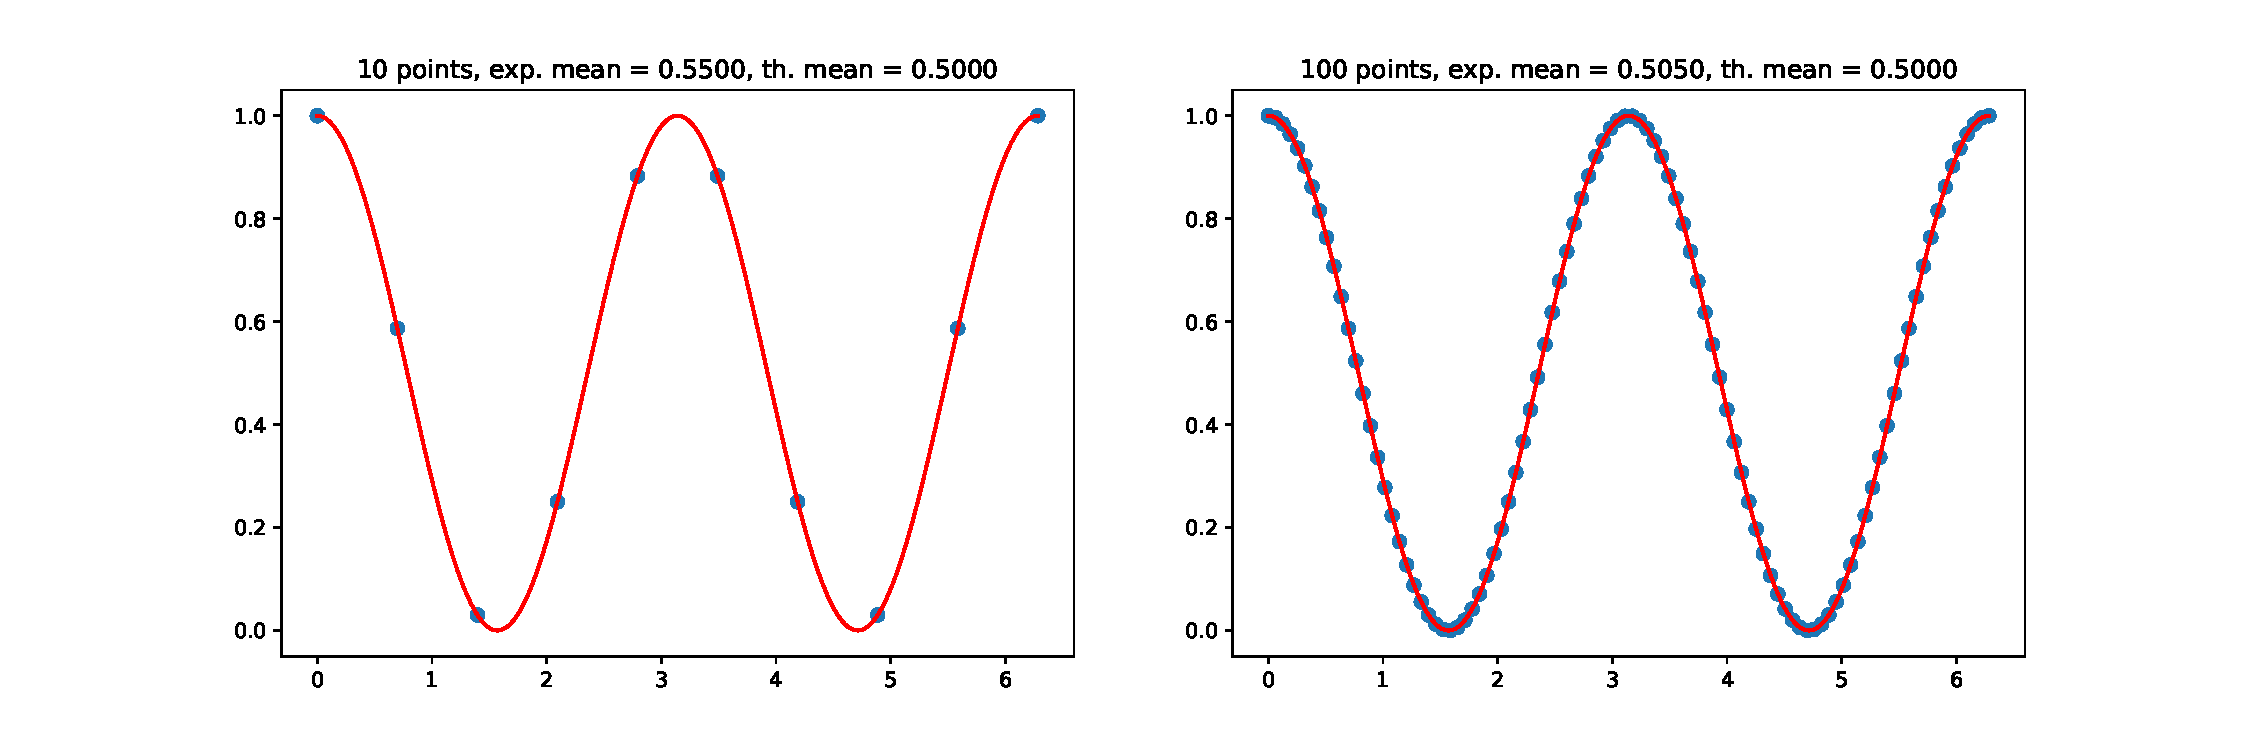
\includegraphics[width=1.5\textwidth]{test.pdf}
    \caption{If we increase the sampling frequency while keeping the interval fixed we can obtain a better representation of the function, which means that the arithmetic average becomes a better approximation of the analytical average.}
    %\label{fig:my_label}
\end{figure}

Indeed if we assume $N=1/\Delta$ and $N$ large we can use the Riemann sum to write:
\begin{equation*}
    \frac{1}{N}\sum_{i=1}^N \cos^2(\omega t_i) = \sum_{i=1}^N \Delta \cos^2(\omega t_i) \approx \int_{t_1}^{t_N}\dd{t} \cos^2(\omega t)
\end{equation*}
One can easily prove (e.g. using the complex representation of the cosine) that $\cos^2 x = (1+\cos(2x))/2$, which yields
\begin{equation*}
    c \approx N \int_{t_1}^{t_N}\dd{t} \quadre{\frac{1}{2}+\frac{1}{2}\cos(2 \omega t)} = \frac{1}{2}N (t_N-t_1)+\frac{N}{2}\eval[\frac{1}{\omega}\sin(\omega t)|_{t_1}^{t_N}
\end{equation*}
The first term evaluates to 
\begin{equation*}
    \frac{1}{2}N (N\Delta - 1\cdot\Delta) = \frac{\Delta}{2}N(N-1) \sim N^2
\end{equation*}
which is indeed an $\omega$-independent constant; the second one is negligible \emph{as long as we work in the high frequency limit}, in which $\omega \to +\infty \implies 1/\omega \approx 0$. One can prove that $s \sim N^2$ similarly.\\
The same line of thought can be used to derive $a \approx 0$:
\begin{equation*}
    a \approx \frac{N}{2} \int_{t_1}^{t_N} \sin(2\omega t) \dd{t} = \frac{N}{2} \eval[-\frac{1}{2\omega}\cos(2\omega t)|_{t_1}^{t_N} \approx 0 \quad \text{(if $\omega \to +\infty$)}
\end{equation*}

\subsection{12.3: Posterior marginalization w.r.t. $B_1$, $B_2$}
In order to obtain the 1-D posterior in $\omega$ we need to derive the complete posterior and integrate it as follows:
\begin{equation*}
    P(\omega | D,I) = \int_{-\infty}^{+\infty}\int_{-\infty}^{+\infty} P(\omega, B_1, B_2|D,I) \dd{B_1}\dd{B_2}
\end{equation*}
Let us then derive the full posterior, which must be integrated as stated above.\\
We already derived the likelihood:
\begin{equation*}
    \L(D|\omega, B_1, B_2) = \frac{1}{(2\pi \sigma^2)^{N/2}}\exp(-\frac{Q}{2\sigma^2})
\end{equation*}
where $Q$ was defined above. If we assume that all model parameters are independent we can factorize the prior as follows:
\begin{equation*}
    P(\omega, B_1, B_2|I) = P(\omega|I)P(B_1|I)P(B_2|I) \propto 1
\end{equation*}
where the last equality holds if we assume uniform priors for everything. This prior allows us to write:
\begin{equation*}
    P(\omega, B_1, B_2|D,I) \propto \L(D|\omega, B_1, B_2)
\end{equation*}
which essentially means that we can marginalize the likelihood itself.
The integral to be computed (up to a constant) therefore is:
\begin{equation*}
    \int_{-\infty}^{+\infty}\int_{-\infty}^{+\infty} \exp(-\frac{1}{2\sigma^2}\tonde{N\overline{d^2}-2B_1 R -2B_2 I +B_1^2c+B_2^2s - 2a B_1 B_2}) \dd{B_1}\dd{B_2}
\end{equation*}
The first of these terms ($N\overline{d^2}$) is a constant w.r.t. $(B_1,B_2)$ and hence can be moved outside the integral (and hidden in the proportionality sign). The remaining terms can be rewritten as the sum of a quadratic form in $(B_1, B_2)$ and a linear one, since $R$, $I$, $c$, $s$ are all functions of $\omega$ only; indeed it's easy to show that the non constant part of the exponent can be rewritten as:
\begin{equation*}
    -\frac{1}{2}\mqty(B_1 & B_2)\mqty(c/\sigma^2 & a/\sigma^2 \\ a/\sigma^2 & s/\sigma^2)\mqty(B_1\\B_2)+\mqty(R/\sigma^2 & I/\sigma^2)\mqty(B_1\\B_2)
\end{equation*}
This allows us to use the gaussian integral formula:
\begin{equation}
    \label{eq:integrale_gaussiano}
    \int_{\R^n} \exp[-\frac{1}{2}\vb{x}^T\mat{A}\vb{x} +\vb{b}^T \vb{x}] \dd[n]{\vb{x}} = \frac{(2\pi)^{n/2}}{\sqrt{\det\mat{A}}}\exp(\frac{1}{2}\vb{b}^T \mat{A}^{-1}\vb{b})
\end{equation}
with $\vb{x} = \mqty(B_1 & B_2)^T \implies n=2$, $\vb{b}=\mqty(R/\sigma^2 & I/\sigma^2)^T$ and
\begin{equation*}
    \mat{A} = \frac{1}{\sigma^2} \mqty(c & a \\ a & s) \implies \mat{A}^{-1} = \mqty(s & -a \\ -a & c)\frac{1}{cs - a^2}
\end{equation*}
Substituting in equation \eqref{eq:integrale_gaussiano} we obtain:\footnote{Notice that in the problem statement a couple of terms were missing, in particular $a\approx 0$ had already been substituted (whereas up to this point no approximation has been made) and the $cs$ factor in the first exponential in the last term was missing - also $1/s$ was mistaken for $1/c$.}
\begin{equation*}
    P(\omega|D,I)\propto \frac{1}{\sqrt{cs-a^2}}\exp(\frac{1}{2\sigma^2}\tonde{R^2 s + I^2 c - 2aRI}) = \frac{1}{\sqrt{cs-a^2}}\exp{\frac{cs}{2\sigma^2} \tonde{\frac{R^2}{c} + \frac{I^2}{s}}}\exp(-\frac{aRI}{\sigma^2})
\end{equation*}

\subsection{12.4: MAP vs DFT}
It's easy to prove $R$ and $I$ are the real and imaginary part of the signal's DFT (it suffices to apply Euler's formula). This means that up to a constant the power spectrum of the signal is 
\begin{equation*}
    \frac{R^2+I^2}{N}
\end{equation*}
Let's use the $a\approx 0$, $c,s\sim N^2$ approximations valid in the high frequency regime in the 1-D marginalized posterior derived above. This posterior becomes proportional to:
\begin{equation*}
    \tonde{\exp(\frac{R^2+I^2}{N})}^{N^3/(2\sigma^2)}
\end{equation*}
We immediately notice that the exponent is equal to the signal power spectrum, which trivially yields that the posterior is maximized by the same $\omega$ that maximizes the DFT.\\
In order to obtain this result we used the gaussian model assumption (i.e. that the likelihood can be factorized in the product of 1D gaussians with known variance $\sigma^2$ and $d_i-f(t_i)$ mean), plus the assumptions that $N$ and $\omega$ are both large numbers.

\subsection{12.5: When to use LSQ fitting?}
We know that in order to be able to use least square fitting one needs to have a MVN likelihood (which we do have) with a mean that depends \emph{linearly} on the model parameters (which isn't our case). This means that in order to be able to use LSQ fitting we would need to replace the trigonometric functions with linear ones; in particular instead of having products of nonlinear functions of our 3 parameters we would need to set $\expval{\varepsilon_i}$ equal to $d_i - a\omega -b B_1 -c B_2$ (where $a$, $b$, $c$ are known constants).\\
Of course one may want to Taylor expand to the first order the trigonometric functions to be able to use LSQ, but this isn't a good idea because even if the $t_i$ happen to be small quantities $\omega$ is by assumption a large one, hence $\omega t_i$ is \emph{not} a number close to zero - hence a first order expansion would be quite inaccurate.











































\end{document}
